

\documentclass[margin=0]{standalone}
\usepackage{tikz}
\usepackage{pgfplots,pgfplotstable}
\usepackage{amsmath,amsfonts,amssymb,xfrac,cancel}
\usepackage{xifthen}
\usepackage{ifthen}
\usepackage{xfp}
\usepackage{tikz-dimline}

\usetikzlibrary{arrows,arrows.meta,bending,calc,decorations,shadings,shadows,shapes,shapes.arrows,shapes.geometric,spy,patterns,backgrounds}
\usepgfplotslibrary{units,fillbetween,groupplots,colorbrewer,colormaps}
\pgfplotsset{compat=newest,
	axis line style={line width=0.8pt},
	every axis/.style = {
		scale only axis,
		width=8cm,height=5cm,
		tick style = {line width=0.8pt,black},
		ticklabel style={scale=0.7},
		major tick length = 1.5mm,
		minor tick length = 0.75mm,
		minor x tick num=1,
		minor y tick num=1,
		xlabel style={scale=0.9},
		ylabel style={scale=0.9},
		zlabel style={scale=0.9},
		%xlabel={Photon energy (eV)}, 
		%    	xticklabel style={
			%    	/pgf/number format/precision=2,
			%    	/pgf/number format/fixed,
			%    	/pgf/number format/fixed zerofill,
			%    },
		yticklabel style={
			/pgf/number format/precision=2,
			/pgf/number format/fixed,
			/pgf/number format/fixed zerofill,
		},
		xtick scale label code/.code={},
	},
	every axis plot/.style={smooth,line width=0.5pt},
	/pgfplots/legend image code/.code={%
		\draw[mark repeat=1,mark phase=1,#1] 
		plot coordinates {
			(0cm,0cm) 
			(0.0cm,0cm)
			(0.0cm,0cm)
			(0.0cm,0cm)
			(0.3cm,0cm)%
		};
	},
}
\pgfplotsset{every axis legend/.style={
		cells={anchor=center},
		inner xsep=1pt,
		inner ysep=1pt,
		nodes={scale=0.7,inner sep=2pt, transform shape},
		draw=none,
		at={(1,1)},
		anchor=north east,
	}
}

\def\algaas{Al$_{x}$Ga$_{1-x}$As }


% \pgfplotstableread[col sep=comma]{/media/labfiles/ruco/phd-ssp/phd-codes/TightBinding/gaas-bands.dat}\bands



%\pgfplotsset{every axis legend/.style={
%cells={anchor=center},
%inner xsep=1pt,
%inner ysep=1pt,
%nodes={scale=0.65,inner sep=2pt, transform shape},
%draw=none,
%at={(1,1)},
%anchor=north east,
%}
%}


%\tikzset{
%	% define shorthand key/style to give spy-on node names
%	Name/.style={
%		every spy on node/.append style={
%			name=#1,
%		},
%	},
%}
%\pgfplotsset{
%cycle from colormap manual style/.style={
%every axis plot/.style={smooth,mark=*,mark options={scale=0.5,fill=none,line width=0.5pt},only marks,line width=0.5pt},
%},
%}




\pgfplotsset{rellenoa/.style={pattern=north west lines,pattern color=gray}}

\newcommand{\errorband}[5]{
	\pgfplotstableread[col sep=comma]{#1}\datatable
	\addplot [name path=pluserror,draw=none,no markers,forget plot]
	table [x={#2},y expr=\thisrowno{#3}] {\datatable};
	
	\addplot [name path=minuserror,draw=none,no markers,forget plot]
	table [x={#2},y expr=\thisrowno{#4}] {\datatable};
	
	\addplot [rellenoa,forget plot,opacity=#5]
	fill between[of=pluserror and minuserror];
	
}


\newcommand{\plotwell}[1]{

	\addplot[name path=A,no markers,smooth,tension=0,red] coordinates {(1,1) (7,1) (7,0) (7+5,0) (7+5,1) (7+5+7,1)};
    
	\addplot[name path=B,no markers,smooth,tension=0,blue,name path=B] coordinates {(1,-1.2) (7,-1.2) (7,-0.5) (7+5,-0.5) (7+5,-1.2) (7+5+7,-1.2)};

	\addplot[#1] fill between [of=A and B];

}
\begin{document}

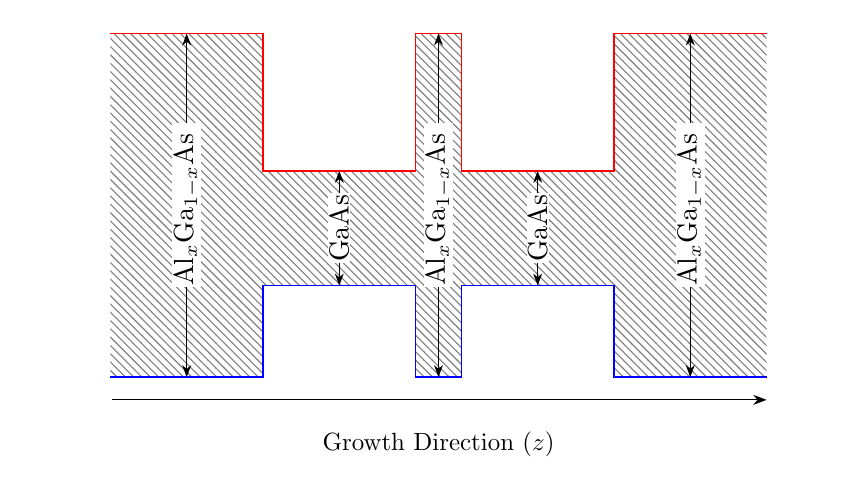
\begin{tikzpicture}
    \begin{axis}[scale only axis,
    	name=edge,
    	anchor=west,
		%yshift=0cm,
        %xshift=0.5cm,
    	%at={(bands001.east)},
    	width=10cm,height=5cm,
        ytick=\empty,
        xtick=\empty,
    	%xtick pos=bottom,
    	%xtick={-4e-2,0,4e-2},
    	%xticklabels={L,$\Gamma$,X},
    	%ylabel={Energy (eV)},
    	xlabel={Growth Direction ($z$)},
    	%xmin=-5e-2,xmax=5e-2,
    	ymin=-0.6,ymax=1.12,
        axis line style={line width=1pt,red,opacity=0},
		]
	

    \def\wbar{10}
    \def\cbar{3}
    \def\wwell{10}
    \def\nwell{10}
    \def\cb{0.6}
    \def\vb{0.4}
    \def\gap{0.5}
	\addplot+[no markers,smooth,tension=0,red,name path=plot1] coordinates 
    {(0,\gap+\cb) 
    (\wbar,\gap+\cb) 
    (\wbar,\gap) 
    (\wbar+\nwell,\gap) 
    (\wbar+\nwell,\gap+\cb) 
    (\wbar+\nwell+\cbar,\gap+\cb)
    (\wbar+\nwell+\cbar,\gap)
    (\wbar+\nwell+\cbar+\wwell,\gap)
    (\wbar+\nwell+\cbar+\wwell,\gap+\cb)
    (\wbar+\nwell+\cbar+\wwell+\wbar,\gap+\cb)};

	\addplot+[no markers,smooth,tension=0,blue,name path=plot2] coordinates 
    {(0,-\vb) 
    (\wbar,-\vb) 
    (\wbar,0) 
    (\wbar+\nwell,0) 
    (\wbar+\nwell,-\vb) 
    (\wbar+\nwell+\cbar,-\vb)
    (\wbar+\nwell+\cbar,0)
    (\wbar+\nwell+\cbar+\wwell,0)
    (\wbar+\nwell+\cbar+\wwell,-\vb)
    (\wbar+\nwell+\cbar+\wwell+\wbar,-\vb)};

    
	\addplot[rellenoa] fill between [of=plot1 and plot2];

		% \node[red] at (axis cs:9.5,0.5){CB};
		% \node[blue] at (axis cs:9.5,-0.75){VB};
	

% \node at (axis cs:\wbar/2,\cb+\gap+0.1) {\algaas};
% \node at (axis cs:\wbar+\nwell+\cbar+\wwell+\wbar/2,\cb+\gap+0.1) {\algaas};
% \node at (axis cs:\wbar+\nwell+\cbar/2,\cb+\gap+0.1) {\algaas};



\dimline[label style={fill=white,scale=1,rotate=180,inner sep=0.2mm},
line style={arrows=Stealth-Stealth,line width=0.1mm},
extension start length=0,
extension end length=0] 
{(axis cs:\wbar/2,\gap+\cb)}
{(axis cs:\wbar/2,-\vb)}
{\algaas};

\dimline[label style={fill=white,scale=1,rotate=180,inner sep=0.2mm},
line style={arrows=Stealth-Stealth,line width=0.1mm},
extension start length=0,
extension end length=0] 
{(axis cs:\wbar+\nwell+\cbar+\wwell+\wbar/2,\gap+\cb)}
{(axis cs:\wbar+\nwell+\cbar+\wwell+\wbar/2,-\vb)}
{\algaas};

\dimline[label style={fill=white,scale=1,rotate=180,inner sep=0.2mm},
line style={arrows=Stealth-Stealth,line width=0.1mm},
extension start length=0,
extension end length=0] 
{(axis cs:\wbar+\nwell+\cbar/2,\gap+\cb)}
{(axis cs:\wbar+\nwell+\cbar/2,-\vb)}
{\algaas};

\dimline[label style={fill=white,scale=1,rotate=180,inner sep=0.2mm},
line style={arrows=Stealth-Stealth,line width=0.1mm},
extension start length=0,
extension end length=0] 
{(axis cs:\wbar+\nwell/2,\gap)}
{(axis cs:\wbar+\nwell/2,0)}
{GaAs};

\dimline[label style={fill=white,scale=1,rotate=180,inner sep=0.2mm},
line style={arrows=Stealth-Stealth,line width=0.1mm},
extension start length=0,
extension end length=0] 
{(axis cs:\wbar+\nwell+\cbar+\wwell/2,\gap)}
{(axis cs:\wbar+\nwell+\cbar+\wwell/2,0)}
{GaAs};
% \dimline[label style={fill=white,scale=1,rotate=-90},
% line style={arrows=Stealth-Stealth,line width=0.1mm},
% extension start length=0,
% extension end length=0] {(axis cs:9.5,-0.5)}{(axis cs:9.5,0)}{$Eg_{\mathrm{B}}$};

\draw[-{Stealth}] (axis cs:0.1,-\vb-0.1)--(axis cs:\wbar+\nwell+\cbar+\wwell+\wbar,-\vb-0.1);
% \node at (axis cs:17,-1.3){$z$};
% \coordinate (cc2) at (axis cs:1,1);
% \coordinate (cc1) at (axis cs:1,-1.2);

\end{axis}


\end{tikzpicture}
\end{document}


